%% Source of figures/empirical-influence.pdf. Compile: pdflatex empirical-influence.tex
%% Generated 2026-10-28 from the SMOTE25 evaluation draft page (76 coded papers, 71 empirical).
%% Numbers are filled from the coded data; regenerate instead of editing them by hand.
\documentclass[border=4pt]{standalone}
\usepackage[scaled]{helvet}\renewcommand{\familydefault}{\sfdefault}
\usepackage{pgfplots}\pgfplotsset{compat=1.18}
\definecolor{sOne}{HTML}{2A78D6}\definecolor{sTwo}{HTML}{EB6834}\definecolor{sThree}{HTML}{1BAF7A}\definecolor{sFour}{HTML}{EDA100}
\definecolor{oZero}{HTML}{A3ABB4}\definecolor{oOne}{HTML}{5598E7}\definecolor{oTwo}{HTML}{1C5CAB}\definecolor{oThree}{HTML}{0D366B}\definecolor{inkTwo}{HTML}{465462}
\begin{document}
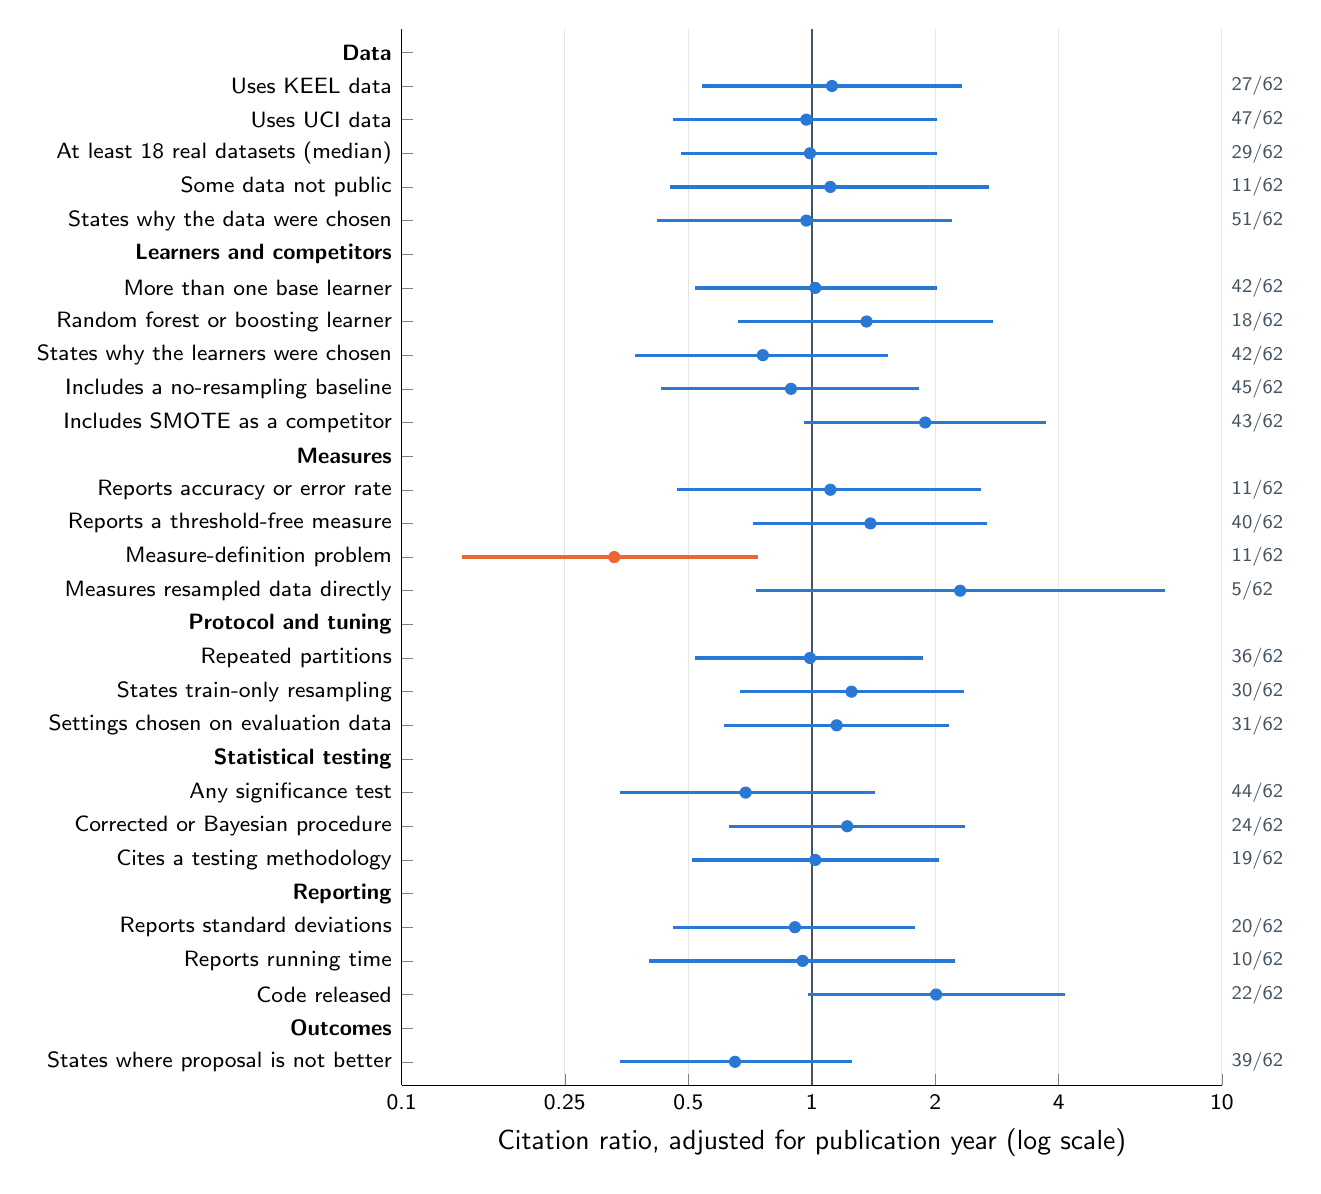
\begin{tikzpicture}
\begin{axis}[xmode=log,log basis x=10,width=12cm,height=15.0cm,xmin=0.1,xmax=10,ymin=-0.7,ymax=30.7,y dir=reverse,
  xtick={0.1,0.25,0.5,1,2,4,10},xticklabels={0.1,0.25,0.5,1,2,4,10},ytick={0,...,30},yticklabels={{\textbf{Data}},{Uses KEEL data},{Uses UCI data},{At least 18 real datasets (median)},{Some data not public},{States why the data were chosen},{\textbf{Learners and competitors}},{More than one base learner},{Random forest or boosting learner},{States why the learners were chosen},{Includes a no-resampling baseline},{Includes SMOTE as a competitor},{\textbf{Measures}},{Reports accuracy or error rate},{Reports a threshold-free measure},{Measure-definition problem},{Measures resampled data directly},{\textbf{Protocol and tuning}},{Repeated partitions},{States train-only resampling},{Settings chosen on evaluation data},{\textbf{Statistical testing}},{Any significance test},{Corrected or Bayesian procedure},{Cites a testing methodology},{\textbf{Reporting}},{Reports standard deviations},{Reports running time},{Code released},{\textbf{Outcomes}},{States where proposal is not better}},
  xlabel={Citation ratio, adjusted for publication year (log scale)},tick label style={font=\footnotesize},y tick label style={align=right},xmajorgrids,grid style={gray!20},axis y line*=left,axis x line*=bottom,clip=false]
\draw[inkTwo,thick] (axis cs:1,-0.7) -- (axis cs:1,30.7);
\draw[sOne,line width=1.2pt] (axis cs:0.54,1) -- (axis cs:2.32,1);\fill[sOne] (axis cs:1.12,1) circle[radius=2.2pt];\node[font=\scriptsize,text=inkTwo,anchor=west] at (axis cs:10,1) {27/62};
\draw[sOne,line width=1.2pt] (axis cs:0.46,2) -- (axis cs:2.02,2);\fill[sOne] (axis cs:0.97,2) circle[radius=2.2pt];\node[font=\scriptsize,text=inkTwo,anchor=west] at (axis cs:10,2) {47/62};
\draw[sOne,line width=1.2pt] (axis cs:0.48,3) -- (axis cs:2.02,3);\fill[sOne] (axis cs:0.99,3) circle[radius=2.2pt];\node[font=\scriptsize,text=inkTwo,anchor=west] at (axis cs:10,3) {29/62};
\draw[sOne,line width=1.2pt] (axis cs:0.45,4) -- (axis cs:2.71,4);\fill[sOne] (axis cs:1.11,4) circle[radius=2.2pt];\node[font=\scriptsize,text=inkTwo,anchor=west] at (axis cs:10,4) {11/62};
\draw[sOne,line width=1.2pt] (axis cs:0.42,5) -- (axis cs:2.2,5);\fill[sOne] (axis cs:0.97,5) circle[radius=2.2pt];\node[font=\scriptsize,text=inkTwo,anchor=west] at (axis cs:10,5) {51/62};
\draw[sOne,line width=1.2pt] (axis cs:0.52,7) -- (axis cs:2.02,7);\fill[sOne] (axis cs:1.02,7) circle[radius=2.2pt];\node[font=\scriptsize,text=inkTwo,anchor=west] at (axis cs:10,7) {42/62};
\draw[sOne,line width=1.2pt] (axis cs:0.66,8) -- (axis cs:2.77,8);\fill[sOne] (axis cs:1.36,8) circle[radius=2.2pt];\node[font=\scriptsize,text=inkTwo,anchor=west] at (axis cs:10,8) {18/62};
\draw[sOne,line width=1.2pt] (axis cs:0.37,9) -- (axis cs:1.53,9);\fill[sOne] (axis cs:0.76,9) circle[radius=2.2pt];\node[font=\scriptsize,text=inkTwo,anchor=west] at (axis cs:10,9) {42/62};
\draw[sOne,line width=1.2pt] (axis cs:0.43,10) -- (axis cs:1.83,10);\fill[sOne] (axis cs:0.89,10) circle[radius=2.2pt];\node[font=\scriptsize,text=inkTwo,anchor=west] at (axis cs:10,10) {45/62};
\draw[sOne,line width=1.2pt] (axis cs:0.96,11) -- (axis cs:3.72,11);\fill[sOne] (axis cs:1.89,11) circle[radius=2.2pt];\node[font=\scriptsize,text=inkTwo,anchor=west] at (axis cs:10,11) {43/62};
\draw[sOne,line width=1.2pt] (axis cs:0.47,13) -- (axis cs:2.59,13);\fill[sOne] (axis cs:1.11,13) circle[radius=2.2pt];\node[font=\scriptsize,text=inkTwo,anchor=west] at (axis cs:10,13) {11/62};
\draw[sOne,line width=1.2pt] (axis cs:0.72,14) -- (axis cs:2.67,14);\fill[sOne] (axis cs:1.39,14) circle[radius=2.2pt];\node[font=\scriptsize,text=inkTwo,anchor=west] at (axis cs:10,14) {40/62};
\draw[sTwo,line width=1.2pt] (axis cs:0.14,15) -- (axis cs:0.74,15);\fill[sTwo] (axis cs:0.33,15) circle[radius=2.2pt];\node[font=\scriptsize,text=inkTwo,anchor=west] at (axis cs:10,15) {11/62};
\draw[sOne,line width=1.2pt] (axis cs:0.73,16) -- (axis cs:7.26,16);\fill[sOne] (axis cs:2.3,16) circle[radius=2.2pt];\node[font=\scriptsize,text=inkTwo,anchor=west] at (axis cs:10,16) {5/62};
\draw[sOne,line width=1.2pt] (axis cs:0.52,18) -- (axis cs:1.87,18);\fill[sOne] (axis cs:0.99,18) circle[radius=2.2pt];\node[font=\scriptsize,text=inkTwo,anchor=west] at (axis cs:10,18) {36/62};
\draw[sOne,line width=1.2pt] (axis cs:0.67,19) -- (axis cs:2.35,19);\fill[sOne] (axis cs:1.25,19) circle[radius=2.2pt];\node[font=\scriptsize,text=inkTwo,anchor=west] at (axis cs:10,19) {30/62};
\draw[sOne,line width=1.2pt] (axis cs:0.61,20) -- (axis cs:2.16,20);\fill[sOne] (axis cs:1.15,20) circle[radius=2.2pt];\node[font=\scriptsize,text=inkTwo,anchor=west] at (axis cs:10,20) {31/62};
\draw[sOne,line width=1.2pt] (axis cs:0.34,22) -- (axis cs:1.43,22);\fill[sOne] (axis cs:0.69,22) circle[radius=2.2pt];\node[font=\scriptsize,text=inkTwo,anchor=west] at (axis cs:10,22) {44/62};
\draw[sOne,line width=1.2pt] (axis cs:0.63,23) -- (axis cs:2.36,23);\fill[sOne] (axis cs:1.22,23) circle[radius=2.2pt];\node[font=\scriptsize,text=inkTwo,anchor=west] at (axis cs:10,23) {24/62};
\draw[sOne,line width=1.2pt] (axis cs:0.51,24) -- (axis cs:2.04,24);\fill[sOne] (axis cs:1.02,24) circle[radius=2.2pt];\node[font=\scriptsize,text=inkTwo,anchor=west] at (axis cs:10,24) {19/62};
\draw[sOne,line width=1.2pt] (axis cs:0.46,26) -- (axis cs:1.79,26);\fill[sOne] (axis cs:0.91,26) circle[radius=2.2pt];\node[font=\scriptsize,text=inkTwo,anchor=west] at (axis cs:10,26) {20/62};
\draw[sOne,line width=1.2pt] (axis cs:0.4,27) -- (axis cs:2.23,27);\fill[sOne] (axis cs:0.95,27) circle[radius=2.2pt];\node[font=\scriptsize,text=inkTwo,anchor=west] at (axis cs:10,27) {10/62};
\draw[sOne,line width=1.2pt] (axis cs:0.98,28) -- (axis cs:4.14,28);\fill[sOne] (axis cs:2.01,28) circle[radius=2.2pt];\node[font=\scriptsize,text=inkTwo,anchor=west] at (axis cs:10,28) {22/62};
\draw[sOne,line width=1.2pt] (axis cs:0.34,30) -- (axis cs:1.25,30);\fill[sOne] (axis cs:0.65,30) circle[radius=2.2pt];\node[font=\scriptsize,text=inkTwo,anchor=west] at (axis cs:10,30) {39/62};
\end{axis}
\end{tikzpicture}
\end{document}
